\chapter{数据源与预处理}

与一般区域水稻遥感制图不同，本研究需要在全球尺度同时服务于水稻生长季识别、全球水稻数据集构建以及稻田与非稻田农田地表温度差异评估。本章将系统说明研究对象、参考数据、遥感数据、土地利用/土地覆盖数据、地表温度数据、地形数据及其预处理流程，明确不同数据在全文证据链中的位置：全球水稻种植差异解释为什么需要开发动态识别方法，参考数据支撑参数选择与精度验证，MODIS地表反射率数据支撑逐日植被指数时间序列构建，土地覆盖数据限定潜在耕地范围，LST和DEM数据则服务于后续稻田地表生物物理降温效应量化。

\section{全球水稻种植概述}

水稻是全球最重要的粮食作物之一，也是受自然条件与人为管理共同控制最强的农田生态系统之一。全球水稻种植集中分布于亚洲季风区，但并不局限于亚洲；非洲西部和东部、南美洲若干平原区、美国南部与加利福尼亚、欧洲地中海沿岸以及澳大利亚灌溉农业区均存在不同规模的稻作系统 \cite{GRiSP2013,Maclean2002,Weng2025}。这种空间分布格局决定了全球水稻遥感监测不能仅以少数典型亚洲稻区为经验基础，而必须面对跨气候区、跨纬度、跨管理制度的复杂对象。

FAO 农业生态区（Agro-Ecological Zones, AEZ）基于热量、水分、地形和生长期等条件，对全球农业生产环境进行综合划分，为理解水稻种植区的自然背景差异提供了基础框架 \cite{FAOAEZ}。从图 \ref{fig:fao_aez} 可以看出，全球农业生态区呈现显著的纬向分异和区域镶嵌特征：热带、亚热带和温带农业生态区在热量条件、生长季长度和水分限制上差异明显，湿润与亚湿润区、半干旱区以及高寒或干旱边缘区又进一步限制了作物生长时段与种植制度。水稻虽然总体上更适宜分布于热量充足、水分条件较好的低地农业生态区，尤其是亚洲季风区、河流三角洲和冲积平原，但在灌溉工程和人为管理支持下，也可延伸至地中海型气候区、温带机械化稻区和部分半干旱灌溉农区。因此，AEZ 图并不是简单给出水稻分布边界，而是用于说明全球稻作系统所处自然背景的高度异质性；这种异质性会通过播栽期、生长季长度、复种制度和水分管理方式传导到遥感时间序列中，成为全球水稻动态识别必须处理的基础约束。

\begin{figure}[htbp]
    \centering
    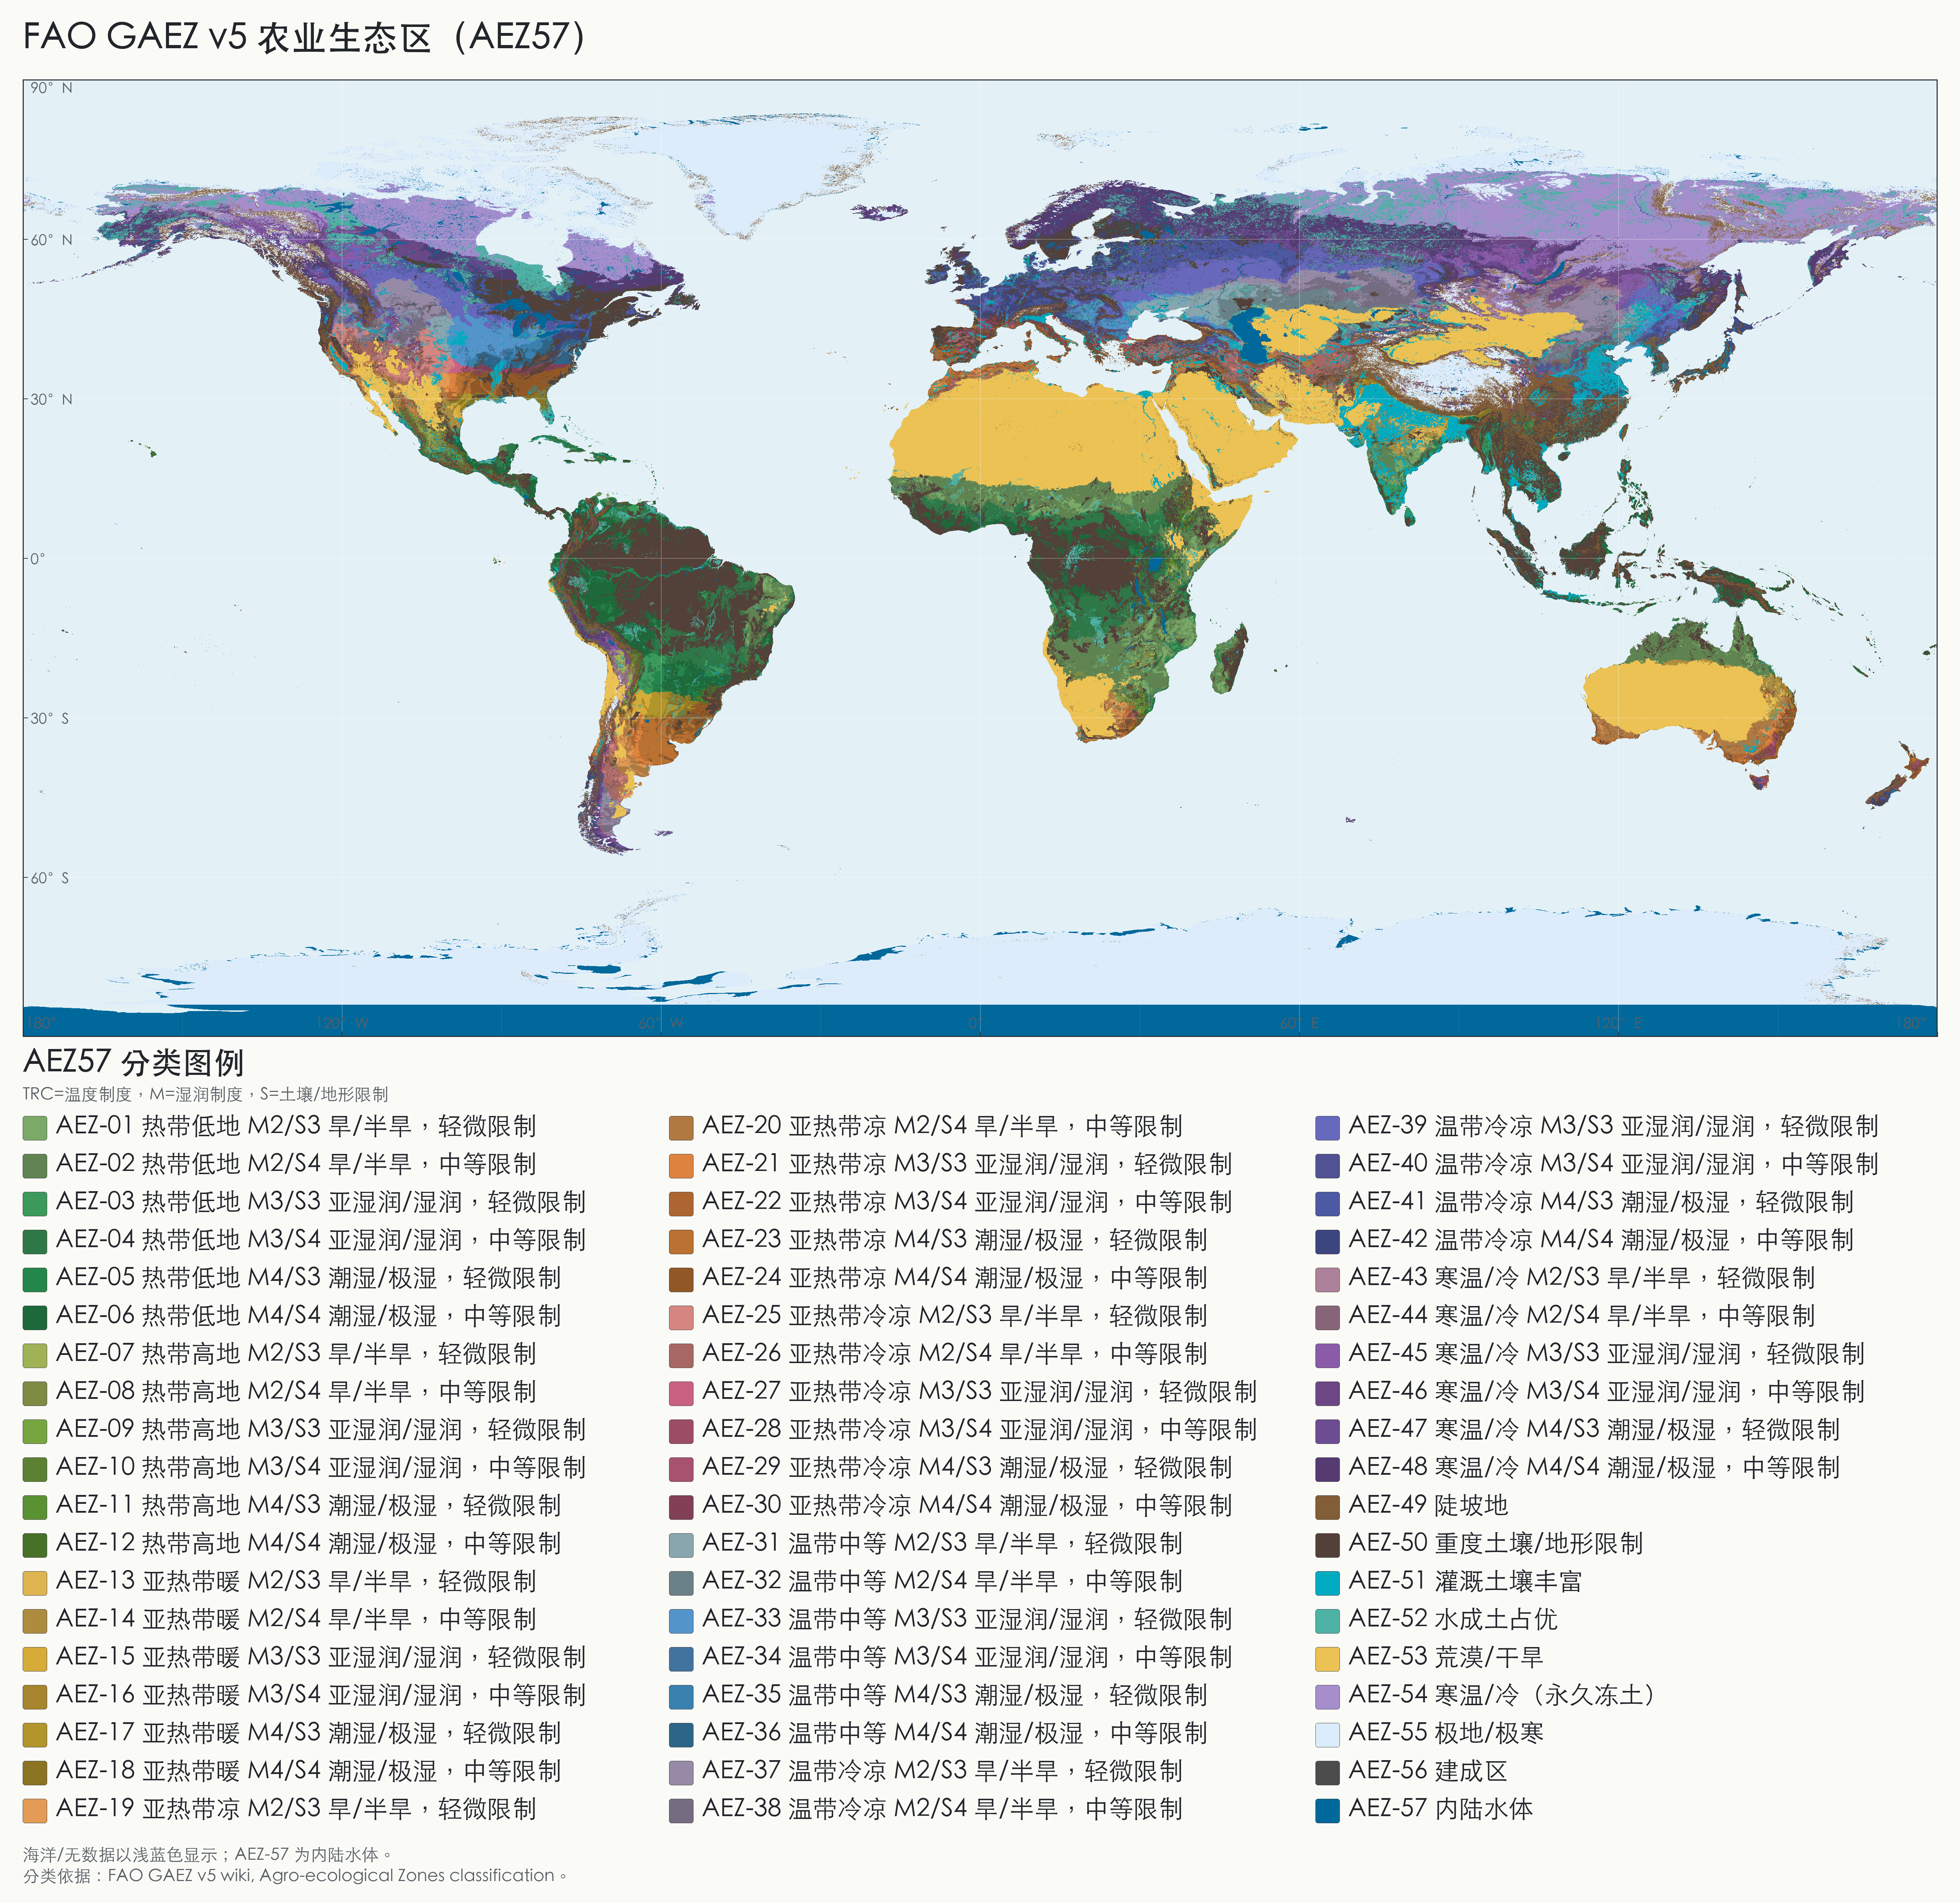
\includegraphics[width=0.99\linewidth]{figure/chapter2/FAO_GAEZ_V5_AEZ57_全球分布图.png}
    \bicaption{FAO农业生态区（AEZ）全球分布}{Global distribution of FAO Agro-Ecological Zones (AEZ)}
    \label{fig:fao_aez}
\end{figure}

从农业生态系统类型看，全球水稻可概括为灌溉低地稻、雨养低地稻、雨养旱地稻以及深水稻或浮稻等主要类型 \cite{GRiSP2013,Maclean2002}。灌溉低地稻通常分布于大型冲积平原、河流三角洲和灌溉条件较好的平坦农区，移栽或返青初期常伴随明显的浅水层，因而在遥感时间序列中更容易出现水分指数升高和植被指数随后快速上升的典型信号。雨养低地稻受季风降水和田间排灌条件影响更强，播栽期往往与雨季到来密切相关，年际波动较大。雨养旱地稻和部分直播稻缺少持续或显著的淹水阶段，其光谱时序可能更接近旱地作物。深水稻和浮稻则与洪泛过程耦合，水位变化本身会改变地表反射率、植被覆盖度和可观测物候阶段。这些生态系统差异使“稻田”在遥感意义上并不是一个固定光谱类别，而是由水层、土壤、植被冠层和管理过程共同构成的动态农田系统。

从区域种植制度看，温带稻区通常以单季稻为主，生长季集中于春末至秋季，播栽期和收获期相对清晰；亚热带季风区常见单季稻与双季稻并存，同一地区可能同时存在早稻、中稻、晚稻和再生稻等不同制度；热带稻区由于水热条件充足，水稻播栽期不再严格受单一温度季节约束，一年内可能出现双季甚至三季水稻，部分水稻季从上一自然年末开始并延续到下一自然年，或在一个自然年内连续衔接多个生长季。由此，热带稻区的水稻识别不仅需要判断某个像元是否种植水稻，还需要准确分离相邻水稻季次、处理跨年生长季归属，并避免将连续种植条件下的物候曲线误合并为一个过长生长季 \cite{Xiao2006,Dong2016,Weng2025}。非洲扩张区的稻田面积增长较快，但地块破碎化、雨养比例高、区域参考数据不足等问题突出；美国、意大利、西班牙、澳大利亚等机械化稻区面积相对有限，但田块形态规整、灌溉管理强、年度种植安排受市场和水资源约束明显。这些差异共同说明，全球水稻制图的关键难点并不只是分类器精度，而是如何在不同播栽期、生长季长度和复种制度的复杂情景下稳定识别真实水稻生长季。

因此，针对全球水稻普适性提取，无法采用固定月份或固定物候窗口来定义水稻生长季。若在全球范围内使用统一的月份窗口，温带单季稻可能被较好覆盖，但热带多熟区会出现错季、漏季或将非生长季纳入分析的问题；若仅依赖区域作物历，非洲、南美洲和热带地区因先验资料不足而难以保持一致性。第二章所整理的数据体系正是为后续 MPD\_DTW 框架服务：利用高时间分辨率 MODIS 地表反射率序列捕捉水稻从淹水、返青、旺盛生长到成熟收获的连续变化，利用参考图和统计数据约束参数与验证结果，并最终生成可支撑地表温度效应评估的日尺度全球水稻动态信息。

\section{参考数据}

本节所述参考数据是支撑本研究参数优选与像元级精度评价的基础数据，主要由来自不同区域、不同来源的局地尺度高分辨率水稻图构成。为提高参考样本对全球水稻种植条件的代表性，本研究在现有资料可得条件下，系统收集并整理了覆盖全球主要产稻区的多源参考数据，包括公开发布的政府数据集、已发表的学术水稻制图产品、区域专题制图资料以及必要的目视解译结果等。综合考虑数据可获取性、空间分辨率、时间一致性、精度水平和区域代表性，最终筛选并采用的参考数据见表 \ref{tab:rice_reference_datasets}。参考数据覆盖中国东北、中国东南、韩国与日本、东南亚、澳大利亚、马达加斯加、意大利伦巴第大区（Lombardy, Italy）、美国以及巴西南里奥格兰德州（Rio Grande do Sul, Brazil）等九个参考区域，涵盖全球所有水稻种植洲，并表征单季稻、双季稻和多季稻等主要稻作制度。这些参考数据能够反映不同洲际背景、气候条件、田块形态、灌溉管理方式和复种制度下的水稻空间分布特征，为全球水稻制图的参数优化与精度验证提供重要数据支撑。

\begin{table}[htbp]
    \centering
    % \small
    \caption{本研究使用的参考数据集}
    \label{tab:rice_reference_datasets}
    \begin{tabular}{@{}m{0.08\textwidth}m{0.14\textwidth}m{0.12\textwidth}m{0.12\textwidth}m{0.25\textwidth}m{0.14\textwidth}@{}}
        \toprule
        大洲 & 参考区域 & 来源类型 & 数据格式 & 数据集或资料名称 & 数据年份 \\
        \midrule
        亚洲 & \makecell[l]{东北亚与\\[-3pt]东南亚} & 以往研究 & 10m栅格 & NESEA-Rice10 \cite{Han2021} & 2017--2019 \\
        亚洲 & 中国东南 & 专题资料 & 30m栅格 & \makecell[l]{中国长江中下游\\[-3pt]水稻数据集} & 2018 \\
        非洲 & 马达加斯加 & 目视解译 & 矢量图斑 & {} & 2019 \\
        欧洲 & \makecell[l]{意大利\\[-3pt]伦巴第} & 官方发布 & 20m栅格 & Carta Uso Agricolo & 2014--2019 \\
        北美洲 & 美国 & 官方发布 & 30m栅格 & Cropland Data Layer\cite{Boryan2011CDL} & 2008--2022 \\
        南美洲 & 巴西 & 官方发布 & 矢量图斑 & \makecell*[l]{Conab \\[-3pt]Mapeamentos \\[-3pt]Agricolas} & 2019 \\
        大洋洲 & 澳大利亚 & 官方发布 & 500m栅格 & \makecell[l]{National scale \\[-3pt]land use data} & 2010 \\
        \bottomrule
    \end{tabular}
\end{table}

\subsection{参考区域简介}

\noindent （1）中国东北。

中国东北参考区覆盖黑龙江、吉林和辽宁境内的主要稻作平原区，包括三江平原、松嫩平原及辽河平原等连片稻田集中分布区。该区域水稻以单季稻为主，机械化和灌溉水平较高，田块相对完整，水稻播栽期和成熟期受春季低温、积温条件和秋季霜冻期约束，具有高纬度、短生长季和物候窗口相对集中的典型特征。

本区域采用 NESEA-Rice10\cite{Han2021} 中覆盖中国东北的 10 m 年度水稻图作为该区域主要参考数据。该数据集基于 MODIS 8 d 地表反射率时序和 Sentinel-1 SAR VH/VV 后向散射时序构建，利用移栽期淹水信号、EVI 生长过程、SAR 后向散射变化以及坡度、森林和湿地掩膜等规则识别稻田，从而在保持较高时间信息的同时降低 500 m MODIS 产品常见的混合像元影响。

\noindent （2）中国东南。

中国东南参考区主要覆盖长江中下游及其邻近的华东、华中和部分华南高强度稻作区，重点服务于中国亚热带复种稻区的空间验证。该区域水热条件优越，河湖水系密集，长期存在单季稻、双季稻以及稻—油、稻—麦等水旱轮作制度并存的格局，是我国稻作制度复杂、复种强度较高的区域之一。该区域水稻地块与河网、湖泊、城镇建设用地、湿地及其他旱作农田高度交错，田块尺度较小，景观破碎化程度和混合像元问题更为突出 \cite{Xiao2005,Zhang2017STOTEN,Wei2022ChinaPaddy}。在长江中下游及其邻近稻作区，稻田淹水信号可能受到河湖湿地、养殖水面、城镇扩张和云雨频繁等因素干扰，因此该区域能够有效检验本文提出的水稻面积提取方法在相邻水稻季、短休闲期、水旱轮作、多熟制背景以及破碎地块边界条件下的适用性。

\noindent （3）日本、韩国与朝鲜。

日本、韩国与朝鲜参考区覆盖日本列岛和朝鲜半岛的主要稻作分布区，其中朝鲜半岛包括韩国和朝鲜两部分，稻田主要分布于西部沿海平原、河谷冲积平原和盆地农区。该区域整体位于东北亚温带季风气候区，水稻以单季稻为主，但田块尺度、地块规整度和农田—居民地镶嵌程度与中国东北大面积连片稻田存在明显差异。韩国西部平原、日本本州沿海平原以及北海道部分平原区稻田物候节律相对集中，灌溉和农田基础设施完善；而韩国和朝鲜部分山地边缘及河谷地区则存在小斑块、窄谷地和破碎农田背景，对稻田识别的空间分辨率和地形适应性提出更高要求。该区域同样采用 NESEA-Rice10 的 10 m 年度水稻图作为参考 \cite{Han2021}。

\noindent （4）东南亚。

东南亚是全球水稻种植最集中、种植制度最复杂的区域之一，典型稻区包括越南红河三角洲和湄公河三角洲、缅甸伊洛瓦底江流域、泰国中部平原、菲律宾北部平原、马来西亚半岛等。东南亚热量条件充足，雨季和旱季转换明显，灌溉稻、雨养低地稻和多季稻广泛并存，单季稻、双季稻和三季稻均有分布。部分热带稻区一年内可出现连续种植或生长季跨自然年的现象，同时云雨频繁也会削弱光学遥感有效观测的连续性\cite{Xiao2006,Sun2023SEAsiaRice20m}。因此，该参考区的作用不仅在于提高亚洲样本覆盖度，更重要的是用于检验本研究的水稻面积提取方法能否适应全年可种植、多峰物候、多季稻和生长季跨自然年的复杂情景。该区域同样采用 NESEA-Rice10 10 m 年度水稻图作为参考 \cite{Han2021}。

\noindent （5）澳大利亚。

澳大利亚水稻种植面积在全球占比较小，但其代表了干旱、半干旱背景下高度依赖灌溉水资源配置的机械化稻作系统，是检验全球水稻制图方法在低水稻占比、稀疏分布和强人为水分调控条件下适用性的重要参考区。澳大利亚水稻主要集中于南部新南威尔士州 Riverina 地区的 Murrumbidgee、Coleambally 和 Murray Valley 等灌溉农业区，另有少量分布于维多利亚州北部、新南威尔士州北部和昆士兰州北部。与亚洲季风区大面积连续稻田不同，该区域田块形态相对规整、机械化水平较高，但空间分布较为稀疏，且年际种植面积高度受灌溉水分配、水市场价格、作物收益预期以及旱涝波动影响。

本研究采用 Australia 2010--11 national scale land use data 作为澳大利亚的参考数据来源。该数据由 Australian Collaborative Land Use and Management Program（ACLUMP）发布，并按照 Australian Land Use and Management Classification（ALUM）体系表达土地利用类型；其中农业用地空间分布综合利用澳大利亚农业普查、MODIS 遥感影像、训练数据以及耕地、园艺和灌溉约束层进行建模。考虑到澳大利亚水稻种植具有显著年际波动，该参考资料主要以土地利用类别和农业作物概率面表达潜在种植分布。

\noindent （6）马达加斯加。

马达加斯加是非洲最具代表性的水稻种植区之一，也是本研究中表征非洲小农稻作系统和复杂地形稻田分布特征的重要参考区域。该国稻作系统类型多样，既包括中央高地的雨养稻和梯田稻，也包括内陆谷地、低洼湿地和灌溉平原稻田，以及部分沿海半淹水稻作区。与亚洲大面积连片稻区和欧美高度机械化稻区相比，马达加斯加稻田受地形起伏、水文条件、灌溉设施和小农经营方式影响更强，田块尺度较小，边界形态复杂，空间破碎化程度较高，公开可用的高分辨率年度水稻参考产品也相对有限。

因此，本研究采用 2019 年目视解译结果作为马达加斯加参考区域数据。该类资料虽然时间覆盖有限、空间范围受解译区域约束，但能够为非洲稻区提供具有较高空间可信度的像元级参考信息，对于弥补非洲水稻验证样本不足、检验算法在复杂地形、小农经营和破碎稻田景观中的识别能力具有重要意义。正式精度评价中，本研究仅将该参考数据用于对应年份和对应空间范围，避免将目视解译结果外推至其他年份或未解译区域，从而降低时间代表性和空间代表性不足带来的验证偏差。

\noindent （7）意大利伦巴第大区。

意大利伦巴第大区位于波河平原，是欧洲最重要的集中连片水稻种植区之一，也是本研究中表征欧洲温带灌溉稻作系统的重要参考区域。该区域水稻主要分布于帕维亚省、Lomellina 以及米兰以南等灌溉农业区，水稻生产以完善的灌溉渠系、较高机械化水平和相对规整的大田块为主要特征。与亚洲季风稻区相比，伦巴第稻田分布更多受波河平原水文条件、灌溉基础设施、欧洲农业经营制度和温带—地中海过渡气候背景共同影响，能够用于检验本研究水稻制图方法在欧洲高管理强度、规则田块和集中连片灌溉稻区中的适用性。

本研究采用 Regione Lombardia 发布的 Carta Uso Agricolo 数据作为伦巴第参考区的数据来源，并选用其中 2014--2019 年覆盖研究时段的水稻类别。该产品基于 SIARL 和 SIS.CO 农业经营档案，对各年度农业用地利用类型进行整理，并包含 ``Riso''（水稻）类别。需要注意的是，官方元数据说明该产品为经重分类和简化后的农业利用图，每个地籍地块主要表达占面积最大的作物或利用类型，局部几何边界可能与实际田块边界存在差异，且不适合直接用于精细作物面积统计。因此，本研究将其作为高分辨率空间参考图使用时，重点保留空间连续、类别明确且与遥感时序特征一致的水稻区域，而不将其直接作为精细地块边界或面积统计真值。

\noindent （8）美国。

美国水稻的主要水稻生产州包括阿肯色、密西西比、密苏里、路易斯安那、得克萨斯和加利福尼亚。与亚洲小农破碎稻区相比，美国稻田田块较大、机械化和灌溉管理水平较高，作物类型记录连续，但不同产区在品种类型、轮作制度和水分管理方式上仍存在差异。美国参考区主要用于检验在长时间序列、机械化灌溉稻作、多作物轮作以及区域化稻作管理背景下的稳定性。

美国参考数据采用 USDA National Agricultural Statistics Service（NASS）发布的 Cropland Data Layer（CDL）2008--2022 年产品。CDL 是年度、地理配准、作物类型化的栅格土地覆盖数据层，基于卫星遥感影像和大量农业地面参考数据生产，2008 年起覆盖美国本土大陆（Continental United States, CONUS），2008--2022 年产品空间分辨率为 30 m，并包含水稻作物类别。CDL 具有年度连续性、作物类别明确和农业训练样本支撑较强等特点，适合作为美国区域长时间序列水稻制图验证的主要参考数据。

\noindent （9）巴西南里奥格兰德州。

巴西参考区位于南里奥格兰德州（Rio Grande do Sul）。该州是巴西灌溉水稻最集中的区域，也是本研究中表征南美洲南半球温带--亚热带灌溉稻作系统的重要参考区。该州稻田主要分布于西部边境区、Campanha、中央区、内外沿海平原和南部低地等灌溉农业区，通常具有灌溉供水、土地平整、田块相对规整和机械化水平较高等特征。

本文采用 Conab/ANA irrigated rice mapping，即 Conab Mapeamentos Agrícolas 中的 ``Arroz Irrigado'' 资料，作为南美洲参考数据来源。该资料面向灌溉水稻农业监测、面积估计和水资源管理，由巴西国家供应公司（Conab）与国家水务和基本卫生署（ANA）等机构合作生产，具有官方制图和区域农业管理背景。

\subsection{参考数据预处理}

参考数据预处理的主要任务是将来源、空间分辨率、类别体系、制图年份和不确定性水平差异显著的多源资料，转化为与本研究的制图单元相匹配的 500 m 像元级参考样本。本研究的制图单元为 500 m 像元，而参考数据多来源于 10--30 m 遥感产品、官方作物图、土地利用资料、作物概率面或目视解译图斑，二者之间存在明显的空间尺度差异。高分辨率参考图能够提供较精细的稻田空间边界，但在聚合到 500 m 尺度时，单个像元内部往往同时包含稻田、田埂、道路、水渠、村落、其他农田及地块边缘等多种地物。若不经过尺度转换和纯度筛选，直接将高分辨率图斑赋值为 500 m 像元级真值，可能导致混合像元被过度确定化，进而影响参数优选和精度评价的可靠性。因此，本研究在预处理阶段从语义一致性、时间一致性和空间尺度一致性等方面对参考资料进行统一处理，以尽可能降低尺度错配、类别歧义和资料不确定性对后续分析的影响 \cite{Dong2016,Weng2025}，参考数据预处理流程见图~\ref{fig:ref_preprocess}。

\begin{figure}[htbp]
    \centering
    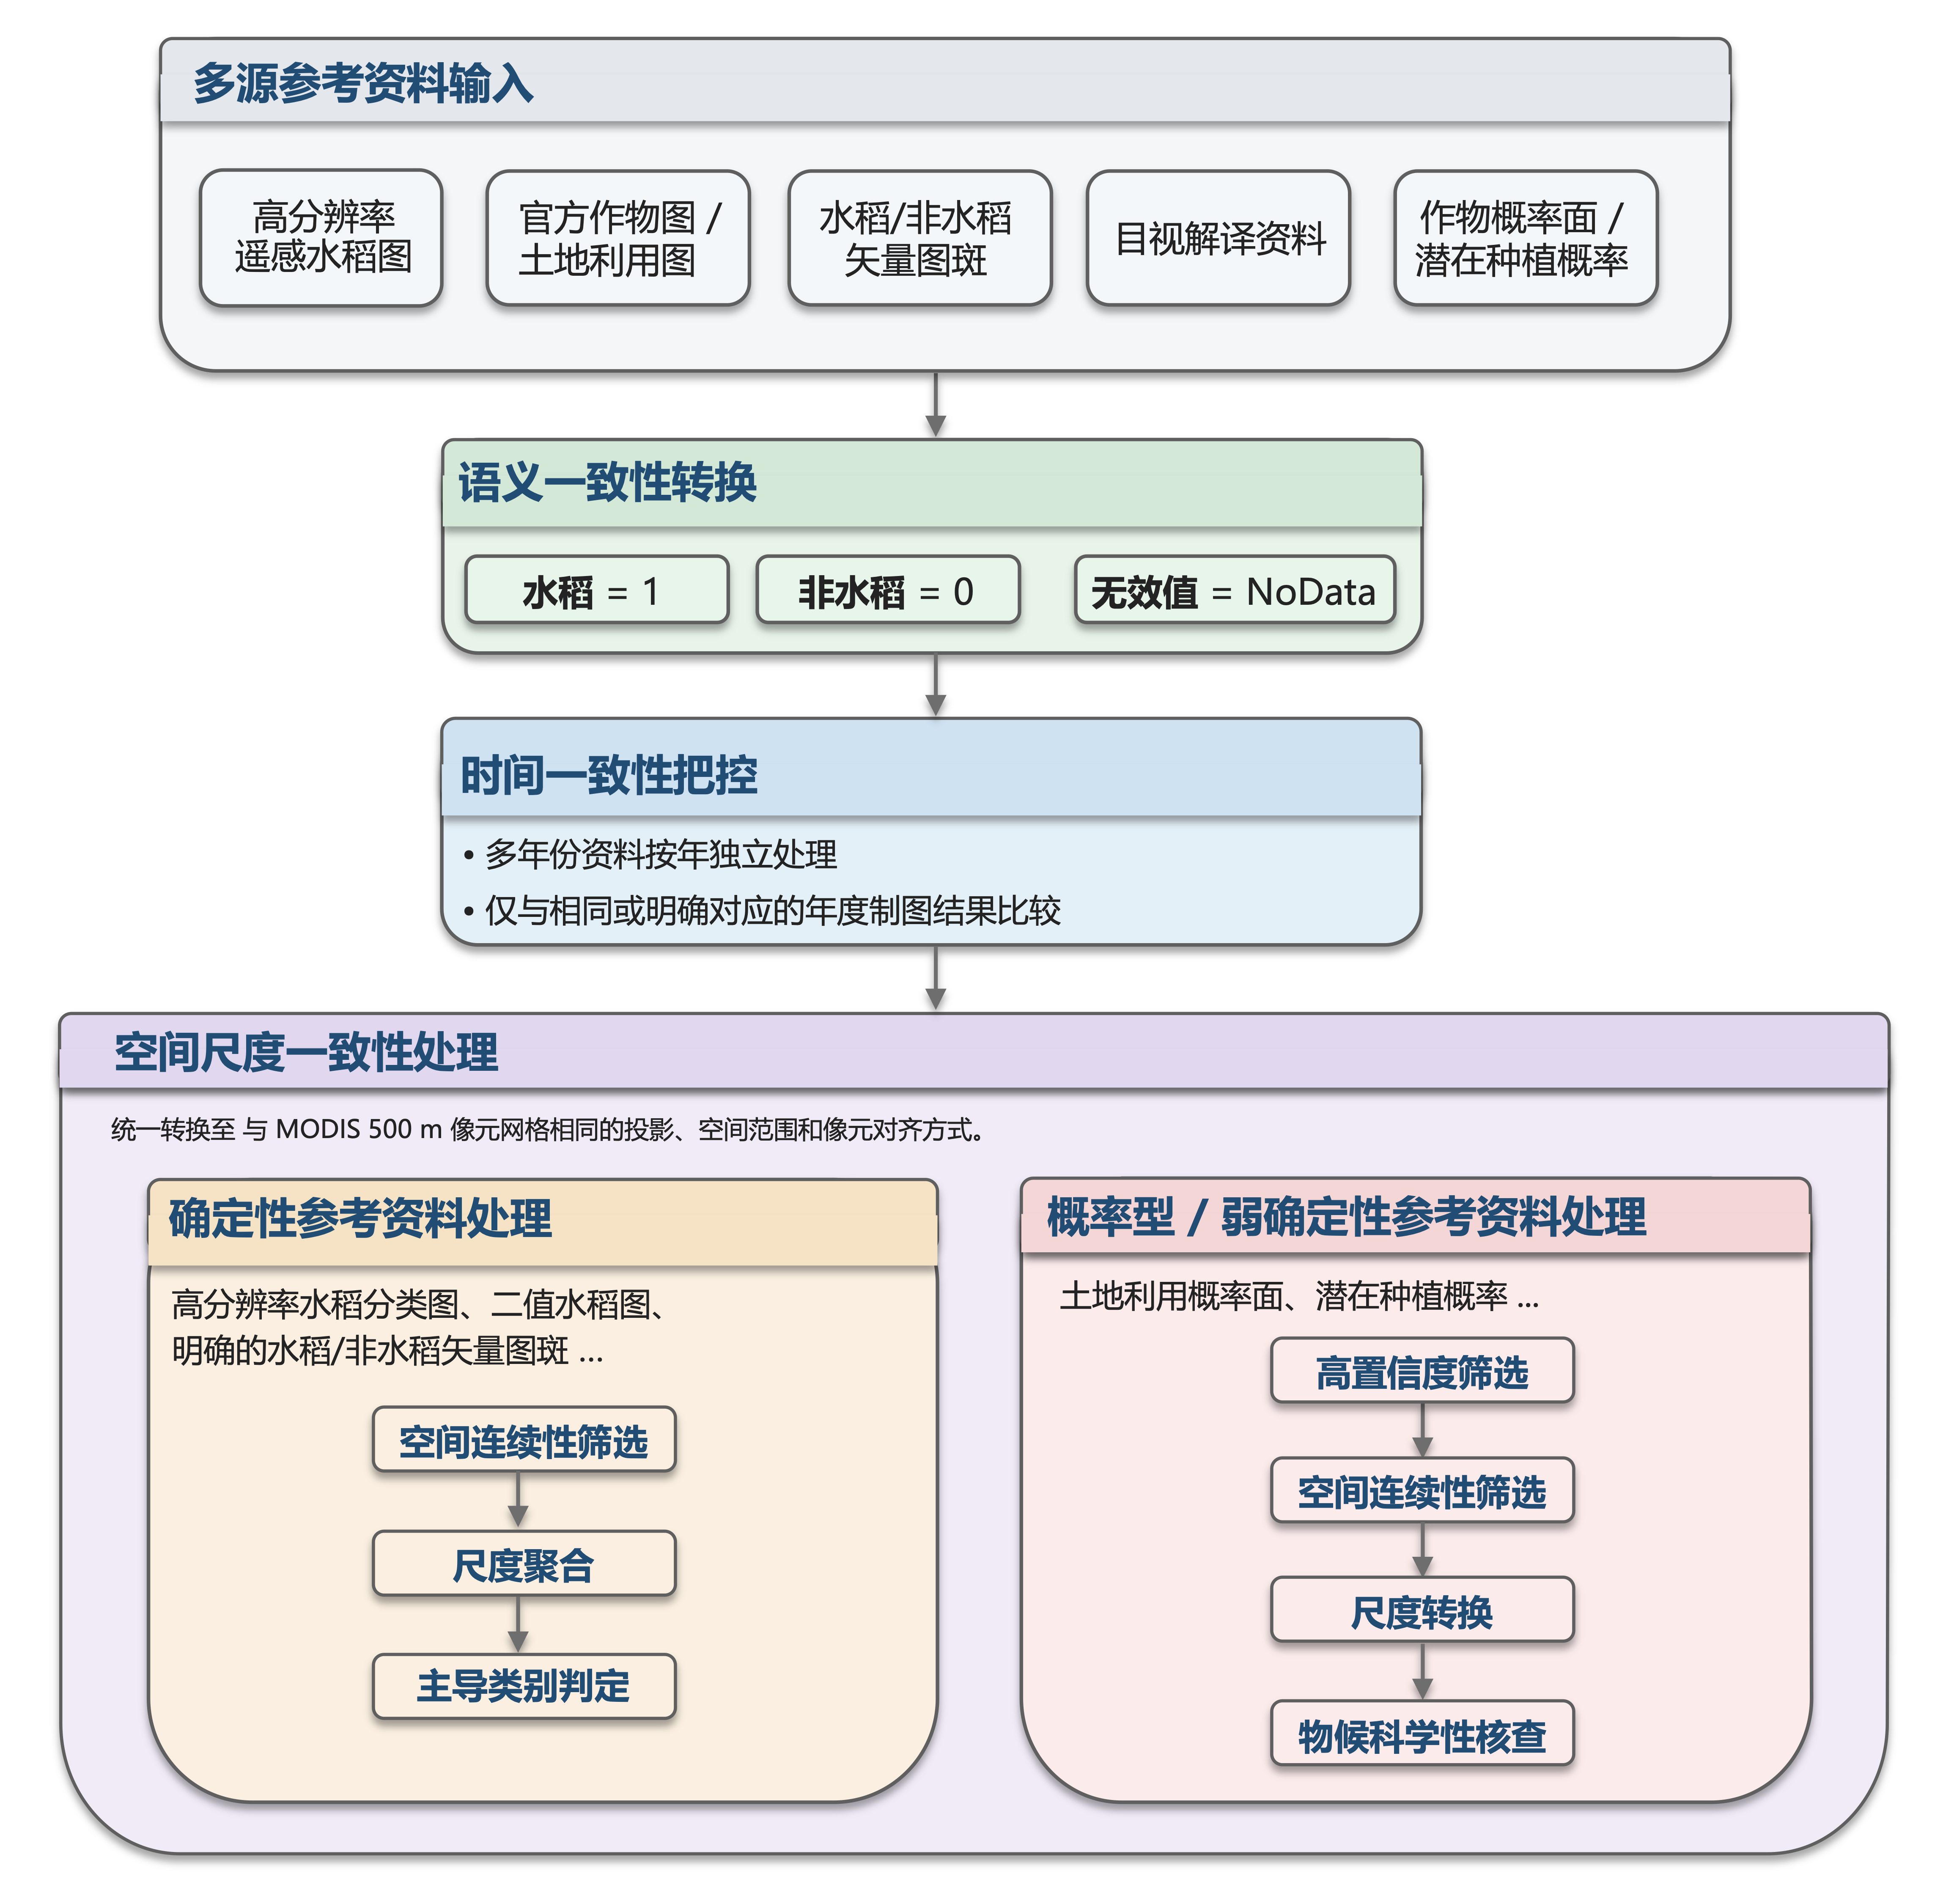
\includegraphics[width=0.95\linewidth]{figure/chapter2/ref_preprocess.png}
    \bicaption{参考数据预处理流程}{Preprocessing workflow for reference data}
    \label{fig:ref_preprocess}
\end{figure}

在语义层面，所有参考资料首先被转换为统一的水稻、非水稻和无效值三类表达，其中水稻像元赋值为 1，明确非水稻像元赋值为 0，研究区外、原始 NoData、类别含义不明确或无法可靠判读的像元赋为无效值。对于具有明确作物类别编码的栅格产品，预处理直接提取水稻类别并保留非水稻背景信息。例如，NESEA-Rice10 中的年度水稻图被用于东北亚和东南亚参考区 \cite{Han2021}，美国 CDL 中提取 rice 类并利用其作物类别体系构建非水稻耕地背景 \cite{Boryan2011CDL}，意大利伦巴第资料提取 ``Riso'' 类，巴西 Conab 资料提取 ``Arroz Irrigado'' 图斑。对于区域专题图和目视解译资料，则依据原始解译范围分别建立正样本和负样本图层，避免将未解译区域默认视为非水稻。上述处理的关键在于区分“明确非水稻”和“未知背景”：前者可进入混淆矩阵评价，后者仅用于空间屏蔽，不能作为检验算法准确性的判据。

在时间层面，多年份参考数据均按年份独立处理，并仅与相同或明确对应的年度制图结果进行比较；单一年份资料只用于其标称年份的空间评价或参数辅助，不外推至其他年份。若源数据包含涵盖多年份，均按年生成独立 tile 文件，以保留作物轮作和年际种植变化。对于南半球或跨自然年生长季，预处理过程将记录资料所对应的播栽年份和收获年份，避免把跨年生长季简单归入错误的日历年。经此处理，参考标签既可以服务于参数选择中对典型物候曲线的提取，也可以服务于按年份开展的空间精度评价。

在空间尺度转换方面，各类参考资料首先统一转换至 MODIS 500 m 像元网格，与本研究所使用的 NDVI 和 LSWI 时间序列使用相同的投影、空间范围和像元网格。

对于高分辨率水稻分类图、二值水稻图、明确的水稻/非水稻矢量图斑资料等确定性参考资料，由于高分辨率参考资料与 MODIS 影像之间存在明显的空间尺度差异，单个 500 m 像元内往往同时包含水稻、其他农田、田埂、水体或建设用地等多种地表组分；若直接采用最近邻重采样，容易将局部高分辨率像元或局部图斑的类别误解释为整个 MODIS 像元的类别，从而放大边界误差和混合像元误差。因此，本研究以 MODIS 500 m 像元内的水稻面积占比作为尺度转换和参考标签生成的基本依据。

在高分辨率尺度上，本研究首先依据原始类别信息对参考资料进行水稻/非水稻识别。对于栅格型参考资料，先将原始分类图转换为水稻与非水稻二值图；对于矢量图斑资料，则根据图斑属性提取明确的水稻图斑和非水稻图斑。在此基础上，进一步进行空间连续性筛选，以剔除孤立斑点、单像元噪声、面积过小的碎片以及类别边界附近不稳定像元。
具体而言，候选水稻或非水稻像元需要满足一定邻域范围内的空间一致性要求，即其周围 $L \times L$ 窗口内应具有足够比例的同类像元，或位于达到最小面积要求的连续斑块内部。经过空间连续性筛选后，仅保留空间结构相对稳定的水稻和非水稻区域，作为后续尺度聚合的基础。

随后，本研究将连续性筛选后的高分辨率参考信息聚合到 MODIS 500 m 尺度。对于栅格型参考资料，分别统计每个 MODIS 像元内连续水稻像元和连续非水稻像元所占面积比例；对于矢量图斑资料，则通过计算水稻或非水稻图斑与 MODIS 像元的空间相交面积，获得对应的水稻面积比例和非水稻面积比例。经过裁剪、重投影、像元对齐和比例聚合后，各类参考资料被统一转换为 500 m 参考比例图。

在参考标签生成阶段，本研究根据 500 m 像元内的面积占比生成水稻、非水稻和无效三类标签。设 $P_{\mathrm{rice}}$ 为 MODIS 500 m 像元内连续水稻区域所占比例，$P_{\mathrm{nonrice}}$ 为连续非水稻区域所占比例，$T_{\mathrm{p}}$ 为主导类别判定阈值，用于判断水稻或非水稻是否构成该 500 m 像元内的主导地表组分。当 $P_{\mathrm{rice}} \geq T_{\mathrm{p}}$ 且不存在明显非水稻信息冲突时，该 MODIS 像元被标记为水稻参考像元；当 $P_{\mathrm{nonrice}} \geq T_{\mathrm{p}}$ 且不存在明显水稻信息冲突时，该像元被标记为非水稻参考像元；当水稻和非水稻比例均未达到阈值，或二者同时满足条件而导致正负样本信息冲突时，该像元被标记为无效值，不参与参数优选和精度评价。

本研究采用 50\% 作为 MODIS 500 m 像元主导类别判定的基础阈值（即 $T_{\mathrm{p}}$ ）。采用 50\% 阈值可以在标签确定性和样本代表性之间取得平衡：一方面，进入评价的像元具有明确的主导类别，避免低比例水稻或低比例非水稻像元被赋予确定性标签；另一方面，该阈值保留了 MODIS 中分辨率制图中普遍存在的混合像元特征，避免参考样本过度集中于大面积、连续且高纯度的稻田斑块。因此，该策略能够使参考样本更接近 GlobalRice500 实际制图尺度下所面对的地表异质性，从而提高参数优选和精度评价的代表性。

本研究所采用的非水稻参考标签仅在源资料能够明确提供非水稻类别、或能够结合可靠耕地掩膜和土地覆盖信息判定非水稻背景时生成。对于仅提供水稻分布范围的二值图或水稻矢量图斑，图斑外区域并不必然等同于可靠的非水稻真值，因此不能简单作为非水稻参考样本使用。通过上述处理，本研究在高分辨率尺度上先控制空间噪声和边界不确定性，再在 MODIS 尺度上进行面积比例聚合和标签判定，从而使参考标签更接近 500 m 像元所观测到的主导地表过程。该策略能够有效降低尺度错配、孤立噪声和混合像元对模型参数优选与精度评价的影响。

对于土地利用概率面或潜在种植概率等概率型或弱确定性参考资料（例如澳大利亚 national scale land use data），为避免低概率区域、边缘性耕地或偶然性土地利用信息被误作为水稻参考标签，本研究在澳大利亚区域采用高置信度阈值、空间连续性筛选和物候科学性核查相结合的策略。首先，仅保留水稻概率或水稻适宜性达到指定阈值的候选像元；其次，剔除空间上孤立或面积过小的候选斑块；最后，结合 NDVI 和 LSWI 时间序列检查其是否具有与水稻生长过程一致的时序特征。

物候科学性核查借鉴 PhenoRice \cite{Boschetti2017RSE}对水稻作物时空物候信息提取的思想，并结合经典水稻遥感制图研究中利用早期淹水信号和后续植被快速生长过程区分水稻与旱地作物的认识\cite{Xiao2005,Xiao2006,Dong2016}。具体而言，本研究重点检查候选像元在水稻移栽、直播出苗或早期淹水阶段是否表现出 LSWI 与 NDVI 的相对关系异常，以及随后是否具有 NDVI 快速上升、峰值形成和成熟期下降等完整生长曲线特征。缺乏水稻生长季时序证据的候选像元被剔除。澳大利亚水稻种植面积占比较低、空间分布相对稀疏，且年度种植范围容易受到灌溉水分配、市场条件和农户管理决策的影响。由于澳大利亚参考数据具有概率型和弱确定性特征，其筛选样本主要用于补充稀疏水稻区的高置信度参考信息。

不同类型参考资料的不确定性来源各异，因此在统一预处理框架下仍需保留针对性质量控制。官方作物图和土地利用图的优势在于类别体系清晰、年度覆盖相对稳定，但其空间边界可能来源于申报地块、地籍单元或农业管理单元，并不一定完全等同于遥感影像中可见的实际田块边界。高分辨率遥感分类产品能够提供较精细的稻田空间信息，但在云雨频繁、地块破碎或淹水信号不明显的区域仍可能存在分类噪声。目视解译资料具有较强的局地可信度，但其空间范围有限，且受影像时相、判读依据和解译人员经验影响。本研究设计的预处理流程，包括三类标签转换、空间连续性筛选和 500 m 主导比例约束，可以有效减少将源数据的边界误差、类别歧义或未判读区域直接传递到参数优选和精度评价中。

经过上述处理后，所有参考数据被组织为统一的年度 MODIS 500 m tile 文件，并保留数据来源、区域名称、年份、纯度阈值、空间分辨率和处理记录。该数据组织方式具有三个直接作用。第一，为后续水稻提取算法等参数优选提供高可信水稻和非水稻样本，使洪水因子、生长季长度约束和 DTW 阈值的设定具有跨区域依据。第二，为像元级精度评价提供与制图结果同网格的参考标签，可直接计算总体精度、用户精度、生产者精度和 F1 分数。第三，它为后续不确定性分析提供可追溯的信息基础，使混合像元、参考数据空间分布不均、资料年份不一致和破碎稻田弱表达等问题能够被明确识别。

\section{统计数据}

本研究中，统计数据主要用于在宏观上进行年度收获面积的一致性检验与校准。与物理稻田面积不同，年度收获面积反映一年内实际完成收获的水稻面积总量；对于非单季稻（双季稻和多季稻）区域，同一像元在一年内被识别为多次水稻收获时，应按收获次数累计像元面积。因此，在与统计数据比较时，本研究将遥感识别结果按照年度收获面积口径进行聚合，以保证遥感解译结果与农业统计口径具有可比性。本文使用的年度收获面积统计数据包括 FAO 国家尺度数据，以及中国、美国和印度的次国家尺度统计数据（表 \ref{tab:rice_statistics_datasets}）。其中，国家尺度 FAO 数据用于评估 GlobalRice500 在全球所有有数据记录的产稻国家的总体面积一致性；中国统计年鉴、美国 USDA 和印度统计年鉴提供了更细行政单元尺度的年度收获面积，可用于检验并校准遥感制图结果在典型大国和主要稻作区内部的区域一致性。后文第 4 章的国家与次国家尺度验证和不确定性讨论均依赖上述统计口径。

\begin{table}[htbp]
    \centering
    \caption{本研究使用的统计数据}
    \label{tab:rice_statistics_datasets}
    \begin{tabular}{ccccl}
        \toprule
        数据来源 & 空间尺度 & 空间范围 & 时间范围 & \multicolumn{1}{c}{网址} \\
        \midrule
        FAO & 国家级 & 全球 & 2001--2022 & \url{https://www.fao.org/faostat/} \\
        中国统计年鉴 & 省级 & 中国 & 2001--2022 & \url{https://www.stats.gov.cn/sj/ndsj/} \\
        美国 USDA & 州级 & 美国 & 2001--2022 & \url{https://www.usda.gov/} \\
        印度统计年鉴 & 邦级 & 印度 & 2009--2016 & \url{https://www.aps.dac.gov.in/} \\
        \bottomrule
    \end{tabular}
\end{table}

\section{遥感数据}

中分辨率成像光谱仪（Moderate Resolution Imaging Spectroradiometer, MODIS）分别搭载于 Terra 和 Aqua 极轨卫星平台，是全球陆表过程、植被动态、水体、积雪、火烧迹地和大气状态监测中应用最广泛的传感器之一。MODIS 具有全球覆盖、长期连续观测、多光谱波段和较高时间重访频率等特点，能够在区域到全球尺度提供稳定一致的陆表遥感时间序列。对于全球水稻制图而言，MODIS 的优势不在于精细刻画田块边界，而在于能够跨越不同气候区和种植制度，持续记录作物生长季内的植被绿度和地表水分变化。

本研究需要在全球尺度开展 20 余年的长时间序列制图，并提取日尺度生长季起止信息；在这一目标下，时间连续性、全球覆盖、长期辐射一致性和计算可行性与空间分辨率同样重要。MODIS 数据能够在全球尺度提供稳定、可更新、长期一致的时序基础，因此，本研究采用 MODIS 500 m 8 日合成地表反射率产品 MOD09A1 和 MYD09A1 作为构建 NDVI 和 LSWI 时间序列的核心遥感数据源。MOD09A1 来自 Terra 卫星，MYD09A1 来自 Aqua 卫星，二者共同提供全球陆地表面反射率长期连续观测。该系列产品自 2000 年以来持续发布并更新，本文选取其中 2000--2023 年的数据用于构建 NDVI 和 LSWI 时间序列，以提取 2001--2022 年的全球水稻面积。

MOD09A1/MYD09A1 提供 7 个 500 m 反射率波段，覆盖可见光、近红外和短波红外等多种波段。表 \ref{tab:mod09a1_bands} 列出了该产品的主要波段、光谱范围及典型敏感信息，其中波长范围依据 MODIS 地表反射率产品用户指南，植被指数和植被水分相关表述参考 MODIS 植被指数及归一化水分指数相关研究 \cite{Vermote2015MOD09UserGuide,Huete2002,Gao1996}。

\begin{table}[htbp]
    \centering
    \caption{MOD09A1/MYD09A1 地表反射率产品主要波段}
    \label{tab:mod09a1_bands}
    \begin{tabular}{cccp{8.8cm}}
        \toprule
        波段 & 光谱名称 & 波长范围（nm） & \multicolumn{1}{c}{主要敏感信息及典型应用} \\
        \midrule
        Band 1 & 红光 & 620--670 & 对叶绿素吸收和裸土--植被差异敏感，常用于植被指数构建、植被覆盖度和作物长势监测。 \\
        Band 2 & 近红外 & 841--876 & 对植被冠层内部散射、叶面积和生物量变化敏感，常用于植被活力、冠层结构和土地覆盖分析。 \\
        Band 3 & 蓝光 & 459--479 & 对大气散射和气溶胶影响较敏感，常用于大气校正、云气溶胶污染辅助识别和真彩色合成。 \\
        Band 4 & 绿光 & 545--565 & 反映绿色植被的可见光反射特征，常用于真彩色合成、植被色调差异和水体/植被背景判读。 \\
        Band 5 & 短波红外 & 1230--1250 & 受植被和土壤含水量影响，常用于地表湿度、积雪/云判别和植被水分状态分析。 \\
        Band 6 & 短波红外 & 1628--1652 & 对液态水吸收和地表干湿条件敏感，常用于植被/土壤水分、积雪和烧毁地识别。 \\
        Band 7 & 短波红外 & 2105--2155 & 对土壤背景、矿物成分、燃烧残留和干湿差异敏感，常用于裸地、烧毁地和地表背景特征分析。 \\
        \bottomrule
    \end{tabular}
\end{table}

本研究主要使用红光、近红外和短波红外波段构建 NDVI 与 LSWI。NDVI 能够表征植被绿度、叶面积指数和生物量变化，是识别水稻返青、旺盛生长和成熟收获过程的主要指标 \cite{Huete2002}。LSWI 对植被冠层和土壤背景中的液态水含量敏感，能够捕捉稻田移栽期或早期淹水阶段的水分信号，因此在水稻遥感识别中具有明确的物理意义 \cite{Gao1996,Xiao2006}。NDVI 与 LSWI 的计算公式如下：
\begin{equation}
    \mathrm{NDVI} = \frac{\rho_{\mathrm{NIR}} - \rho_{\mathrm{red}}}{\rho_{\mathrm{NIR}} + \rho_{\mathrm{red}}}
\end{equation}
\begin{equation}
    \mathrm{LSWI} = \frac{\rho_{\mathrm{NIR}} - \rho_{\mathrm{SWIR}}}{\rho_{\mathrm{NIR}} + \rho_{\mathrm{SWIR}}}
\end{equation}
其中，$\rho_{\mathrm{red}}$、$\rho_{\mathrm{NIR}}$ 和 $\rho_{\mathrm{SWIR}}$ 分别表示红光、近红外和短波红外波段的地表反射率。本研究采用 8 日尺度 MODIS 地表反射率序列构建植被指数，并同步记录观测对应的年积日，为后续逐日移动物候检测提供时间坐标。

由于云、云阴影、气溶胶和降雨会显著影响光学反射率观测，遥感时间序列在进入水稻识别算法前必须进行质量控制和时序重建。对 NDVI 而言，本研究对 MOD09A1 与 MYD09A1 计算得到的 NDVI 在每个 8 日窗口内进行最大值合成，以降低云雨污染对植被绿度估计的影响 \cite{Weng2025}。最大值合成基于一个基本事实，即云和大气污染通常会降低可见光和近红外反射率组合下的植被指数，而生长季真实植被峰值更容易在多次观测中保留下来。对 LSWI 而言，稻田早期淹水信号对水稻识别极为关键，若简单采用最大值或强平滑处理，可能削弱短时淹水特征。因此，本研究保留所有可用 LSWI 观测，并通过后续插值形成日尺度序列 \cite{Weng2025}。

为获得可支持逐日 SOS 和 EOS 搜索的连续植被指数序列，本研究进一步将 8 日尺度 VI 序列重建为日尺度序列。其中，NDVI 采用 Savitzky--Golay 滤波进行平滑重建，以在抑制噪声的同时保留返青、峰值和收获下降等关键物候形态；LSWI 采用线性插值形成连续日尺度序列，以尽量保持淹水信号的时间位置和变化幅度 \cite{Weng2025}。这种差异化处理体现了两类指数在水稻识别中的功能差别：NDVI 更侧重描述完整生长季曲线形态，适合平滑后用于 DTW 曲线匹配；LSWI 更侧重识别移栽或淹水事件，过度平滑可能导致 SOS 判断偏移。

首先，下载并整理 2000--2023 年 MOD09A1 和 MYD09A1 地表反射率数据，提取红光、近红外和短波红外波段，计算 NDVI 与 LSWI，并保留观测对应的年积日信息。随后，根据 MODIS 质量标识和时间序列特征对异常观测进行筛选；NDVI 通过 Terra 与 Aqua 8 日最大值合成降低云雨污染影响，LSWI 则尽可能保留全部有效观测以维持淹水信号完整性。在此基础上，NDVI 采用 Savitzky--Golay 滤波重建为日尺度平滑序列，LSWI 采用线性插值生成日尺度序列。处理后的 NDVI 和 LSWI 构成第 3 章 MPD\_DTW 框架的直接输入，其中 LSWI 主要用于 SOS 淹水条件判断，NDVI 主要用于 EOS 判断和 DTW 曲线匹配。

\section{土地利用/土地覆盖数据}

土地利用/土地覆盖数据主要用于构建全球水稻潜在搜索范围和后续稻田降温效应评价中的非稻田农田候选区域。水稻遥感识别若在全球所有陆地像元上直接进行，不仅计算量巨大，而且容易将湿地、水体边缘、水生植被或季节性淹水裸地误判为稻田。通过耕地掩膜预先排除明显非农业地表，能够提高计算效率并降低非耕地湿润背景带来的误判风险。但需要强调的是，耕地掩膜并不是水稻分类结果本身，而是为 MPD\_DTW 提供合理的候选空间约束。

本研究使用三类土地覆盖产品构建耕地掩膜：MCD12Q1 Land Cover Type 1 中的 IGBP 分类，时间范围为 2001--2022 年；GlobeLand30 2010 年产品；以及美国农业部 Cropland Data Layer（CDL），时间范围为 2008--2022 年 \cite{Boryan2011CDL,Weng2025}。其中，MCD12Q1 具有与 MODIS 时序数据一致的空间尺度和长期年度更新优势，适合作为全球基础耕地信息；GlobeLand30 提供更高空间分辨率的耕地边界信息，可补充 MODIS 土地覆盖产品在破碎农区的表达能力；CDL 在美国具有作物类型细分和年度连续优势，因此被用于美国区域的耕地掩膜构建。

在空间处理上，GlobeLand30 和 CDL 均被重采样至 500 m MODIS tile 格式，并保留耕地比例不低于 50\% 的像元 \cite{Weng2025}。对于美国区域，本研究采用重采样后的 CDL 耕地作为耕地掩膜，以充分利用其作物类型分类精度和年度一致性。对于美国以外区域，则采用 MCD12Q1 IGBP 耕地类别与 GlobeLand30 耕地类别的并集作为耕地掩膜。采用并集而非交集的原因在于，全球水稻制图更需要避免将潜在稻区过早排除；若使用过于严格的交集掩膜，可能在非洲、东南亚丘陵区或破碎小农区造成系统性漏检。与此同时，后续 MPD\_DTW 的物候检测和曲线匹配仍会进一步筛选真实水稻像元，因此耕地掩膜的功能应理解为“尽量完整的候选域约束”，而非最终分类判据。

土地覆盖数据还服务于第 6 章的降温效应量化。稻田地表温度效应的比较对象应尽量限定为周边非稻田农田，而不应直接与城市、森林、水体或裸地比较，否则温度差异会同时混入下垫面类型、粗糙度、反照率和人为热排放等多重因素。本章对耕地掩膜的说明为后续样本匹配奠定基础：只有在同一农田背景内比较稻田与非稻田农田的 LST，才能更接近稻田水分管理和水稻冠层过程本身的生物物理温度效应。

预处理：利用 MCD12Q1、GlobeLand30 和 CDL 构建全球耕地候选域，并将土地覆盖数据统一到 500 m MODIS tile 格式。对于高分辨率土地覆盖产品，先按耕地比例进行聚合，再保留耕地比例不低于 50\% 的像元。该步骤将全球搜索范围约束在潜在农田区域内，为水稻识别减少明显非耕地干扰。与此同时，对全球高分辨率水稻参考图、官方区域水稻产品和目视解译样本进行格式统一、空间聚合和标签筛选，使其与 500 m MODIS 网格一致。统计数据则按照国家或次国家行政单元和年度收获面积口径整理，用于后续遥感面积聚合结果的独立检验。

\section{地表温度数据}

地表温度数据主要用于稻田地表生物物理降温效应的量化。本研究采用 2003--2020 年全球无缝 1 km 日尺度 LST 数据集，该数据集包含白天 13:30 和夜间 01:30 两个时相的地表温度信息 \cite{Weng2025}，能够较好地满足长时间序列、全球覆盖和昼夜对比分析的需求。白天地表温度主要受太阳辐射输入、地表蒸散发、土壤水分和显热/潜热分配控制，对稻田水层蒸发和水稻冠层蒸腾更为敏感；夜间太阳辐射消失后，地表温度差异更多反映热惯性、土壤水分和长波辐射过程。将昼间和夜间 LST 分开处理，是识别稻田降温效应昼夜不对称特征的前提。

LST 数据的时间范围为 2003--2020 年，短于 GlobalRice500 的 2001--2022 年。这一差异来自地表温度数据可用年份与质量控制要求，而不是水稻数据集本身的时间限制。因此，本文在水稻时空动态分析中使用 2001--2022 年 GlobalRice500，而在稻田降温效应分析中使用二者交集范围内的 2003--2020 年。后续所有关于 $\Delta$LST 的多年平均、年际变化和不确定性分析均应以这一时间范围为准，避免将 GlobalRice500 的完整年份误用于 LST 分析。

空间匹配方面，原始 LST 数据空间分辨率为 1 km，而 GlobalRice500 和 MODIS 地表反射率序列采用约 500 m MODIS tile 格式。为实现像元级或局地窗口尺度的稻田与非稻田农田比较，LST 数据被重采样至 500 m MODIS tile 格式，与 GlobalRice500 保持一致 \cite{Weng2025}。这一处理提高了不同数据层之间的空间叠置一致性，但并不意味着 LST 的原始有效空间信息被提升到 500 m。第 6 章和第 8 章在解释田块尺度降温效应时，应始终注意 1 km LST 与 500 m 稻田数据匹配可能引入的邻近效应和混合像元不确定性。

预处理：将 2003--2020 年 1 km 日尺度 LST 数据和 GVE DEM 数据重采样到 500 m MODIS tile 格式，与 GlobalRice500 在空间上保持一致。对于 LST 数据，分别保留白天和夜间时相，并在后续降温效应分析中仅使用水稻真实生长季内的有效温度观测。对于 DEM 数据，则主要提取海拔信息，用于构建稻田与非稻田农田样本之间的地形约束。至此，第二章形成了支撑全文的标准化数据基座：一方面，它为第三章提供可逐日搜索的水稻物候时间序列；另一方面，它为第四章和第五章提供验证与统计分析基础；同时，它为第六章和第七章在真实生长季内量化稻田地表降温效应提供了空间和时间匹配条件。

\section{DEM数据}

数字高程模型用于控制稻田与非稻田农田样本之间的地形差异，减少由海拔差异造成的 LST 偏差。本研究采用 Global Version Elevation（GVE）DEM 数据，并将其重采样至 500 m MODIS tile 格式，与 GlobalRice500 和 LST 数据保持空间一致 \cite{Weng2025}。DEM 在本文中的核心作用并不是直接参与水稻识别，而是在稻田降温效应评估中用于筛选地形条件相近的非稻田农田对照样本。

地形控制对于全球稻田 LST 比较具有必要性。稻田通常分布于平原、河谷、三角洲和低缓丘陵地区，但在东南亚、中国南方、马达加斯加和部分非洲山区也存在梯田或山地稻作。若稻田像元与非稻田对照像元之间存在显著海拔差异，则二者的 LST 差异可能部分来自气温垂直递减率、坡向、太阳辐射几何条件或冷空气汇聚，而不完全来自稻田水分管理和冠层过程。为降低地形差异对温度比较的干扰，后续降温效应量化中要求稻田与非稻田农田之间的海拔差异小于 50 m，并设置距离和样本量约束 \cite{Weng2025}。本章对 DEM 数据的处理说明，为后续样本匹配和不确定性分析提供数据基础。


综合上述数据源，本研究的数据预处理流程可概括为“原始遥感数据整理、质量控制与指数构建、日尺度时序重建、耕地候选域约束、参考数据标准化、统计数据整理、LST 与 DEM 空间匹配”七个环节，如图所示。该流程的设计目标是将空间分辨率、时间范围、投影格式和数据口径各不相同的多源数据，转化为可被第 3 章 MPD\_DTW 方法、第 4 章 GlobalRice500 精度评价、第 5 章全球水稻时空格局分析以及第 6--7 章稻田降温效应评估共同调用的一致数据体系。

